%mainfile: ../../master.tex
\subsection{Ultrasonic Sensor}\label{sub:ultrasonic}

Ultrasonic sensors can be based on different physical principles. Different principles allow for measuring different properties. The following list specifies 3 physical principles and the properties they measure.

\begin{itemize}
  \item time of flight - for measuring a distance, thickness or integrity\cite{ultrasound2}
  \item the Doppler effect - for measuring speed\cite{ultrasound}
  \item the attenuation of sound waves - for measuring distance or directionality\cite{ultrasound}
\end{itemize}

The sensor \enquote{HC-SR04} in consideration is utilising the time of flight principle. This sensor emits a high-frequency (40 kHz) pulse. It then measures the time it takes for an echo of the pulse to reflect back. The sensor has 2 openings on the front. One opening emits ultrasonic waves, thereby acting as a transmitter. The other opening receives the reflected waves, thereby acting as a receiver. \Cref{fig:ultrasonicwiring} illustrates how the sensor is wired to an Arduino device.

\begin{figure}[htbp]
  \centering
  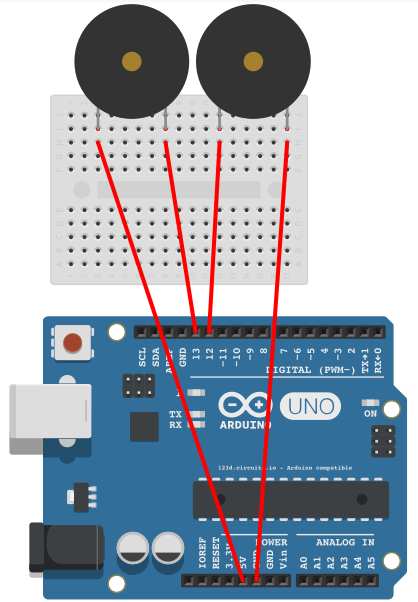
\includegraphics[angle=-90, width=0.6\textwidth]{arduino-ultrasonic-wiring.png}
  \caption[The setup of the ultrasonic sensor testbed]{The setup of the ultrasonic sensor testbed. The 2 speakers on the figure should symbolise an ultrasonic sensor.}\label{fig:ultrasonicwiring}
\end{figure}

\paragraph{Operation of the Sensor}
The \enquote{HC-SR04} sensor operates by the following description. This is also visually represented in \cref{fig:sensor-workings}. First the sensor's measuring mechanism is activated by setting the \enquote{TRIGGER} pin to high for 10$\si{\micro\second}$. Then the sensor begins the measuring cycles consisting of 8 consecutive transmit-receive periods. At last the sensor outputs the time it took for an ultrasonic wave to be transmitted and received again. This can be measured through the \enquote{ECHO} pin. The \enquote{ECHO} pin is HIGH for some time, which can be converted into a distance by the following formula $L = \frac{C \times T}{2}$, where $L$ is the distance, $C$ is the speed of sound, $T$ is the time it took for the wave to travel back and fourth, hence also why we divide by 2.

\begin{figure}[htbp]
  \centering
  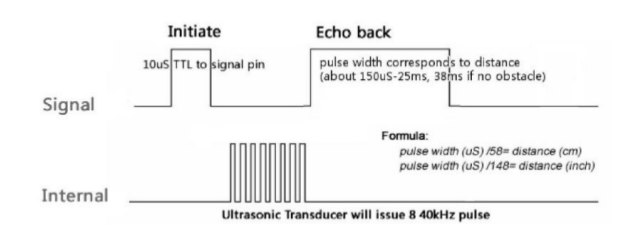
\includegraphics[width=\textwidth]{sensor-workings.png}
  \caption[HC-SR04 timing diagram]{HC-SR04 timing diagram. First, the \enquote{TRIGGER} pin is set HIGH for 10$\si{\micro\second}$. Internally, the sensor will then do 8 cycles of transmit-receive. Finally, the \enquote{ECHO} pin is set HIGH, for the user of the sensor to measure.}
  \label{fig:sensor-workings}
\end{figure}

\paragraph{The Technology}
Ultrasonic sound waves have a number of properties that make them suitable for measurements, that would not be possible with lower frequency waves. Additionally, the waves do not alter the environment it is measuring.

\begin{itemize}
\item Ultrasonic sound waves are inaudible to humans, so they do not affect the behaviour of humans
\item As frequencies of waves increase, so does the attenuation. This means that the rate of attenuation describes the distance the waves have been travelling
\item As the frequencies of waves increase, the reflectiveness of the waves are higher, so more of the waves are reflected back to the sensor 
\end{itemize}

When using the technology, the following considerations should be taken into account.

\begin{itemize}
  \item Temperatures and humidity affect the speed of sound in air
  \item Temperature variations and air currents can act as invisible boundaries that will reflect ultrasonic waves
  \item The angle of the objects being observed. For the transmitted wave to be echoed back to the receiver, the surface of the target must be near perpendicular to the transmitter. I.e. the angle of the object with respect to the sensor does not exceed a particular range
  \item Pulsing ultrasonic sensors may have a \enquote{dead zone} immediately in front of them, in which objects will be detected incorrectly. This may happen because the waves will reflect back to the receiver before it is operational
  \item Some materials may be more absorbent than others, and will therefore reflect less ultrasonic waves
\end{itemize}

\paragraph{The Purpose}
The purpose of the ultrasonic sensor in this project is to figure out if a person is at a specific location in the problem domain e.g. sitting in the sofa watching TV. The PIR sensor described in \cref{sub:pir}, is only capable of sensing motion. The ultrasonic sensor described in this section is capable of measuring a distance to an specific object e.g. a person. The distance is measured every second, so where the PIR sensor would not be capable of tracking a person if the person is not moving, the ultrasonic can detect a person by a change in the distance.

\paragraph{The Tests} The tests of the sensors will include some aspects of the considerations mentioned above, also some tests on the values mentioned in the HC-SR04 datasheet\cite{hcsr04}. The tests will be performed on 3 identical HC-SR04 sensors. The pictures \crefrange{fig:ultra1}{fig:ultra3} depicts how the tests were carried out.

\begin{figure}[htbp]
  \begin{subfigure}{.3\textwidth}
    \centering
    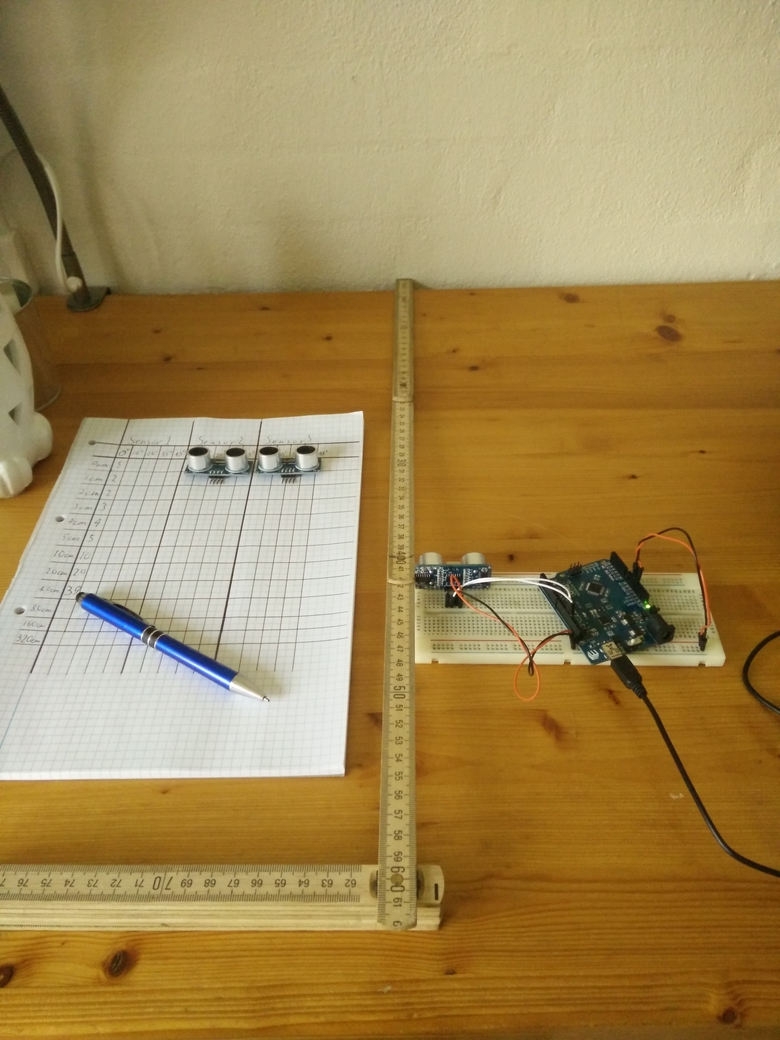
\includegraphics[width=\textwidth]{ultra1.jpg}
    \caption{bla\sinote{ordentlig caption}}
    \label{fig:ultra1}
  \end{subfigure}
  \begin{subfigure}{.3\textwidth}
    \centering
    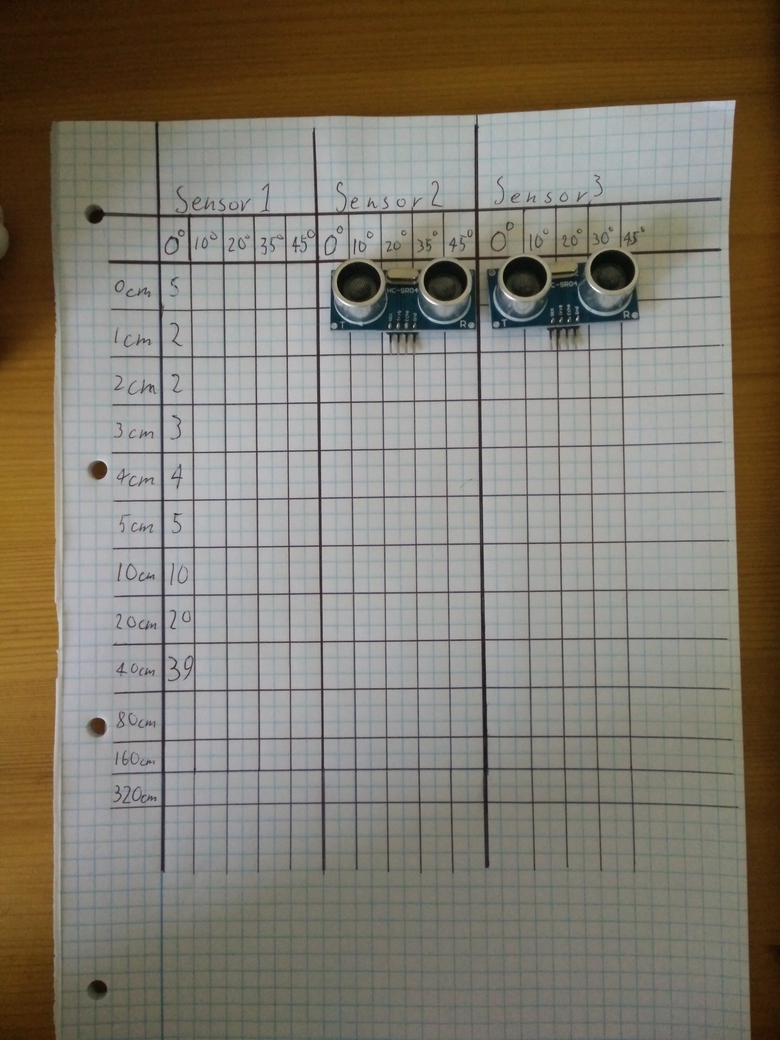
\includegraphics[width=\textwidth]{ultra2.jpg}
    \caption{bla\sinote{ordentlig caption}}
    \label{fig:ultra2}
  \end{subfigure}
  \begin{subfigure}{.3\textwidth}
    \centering
    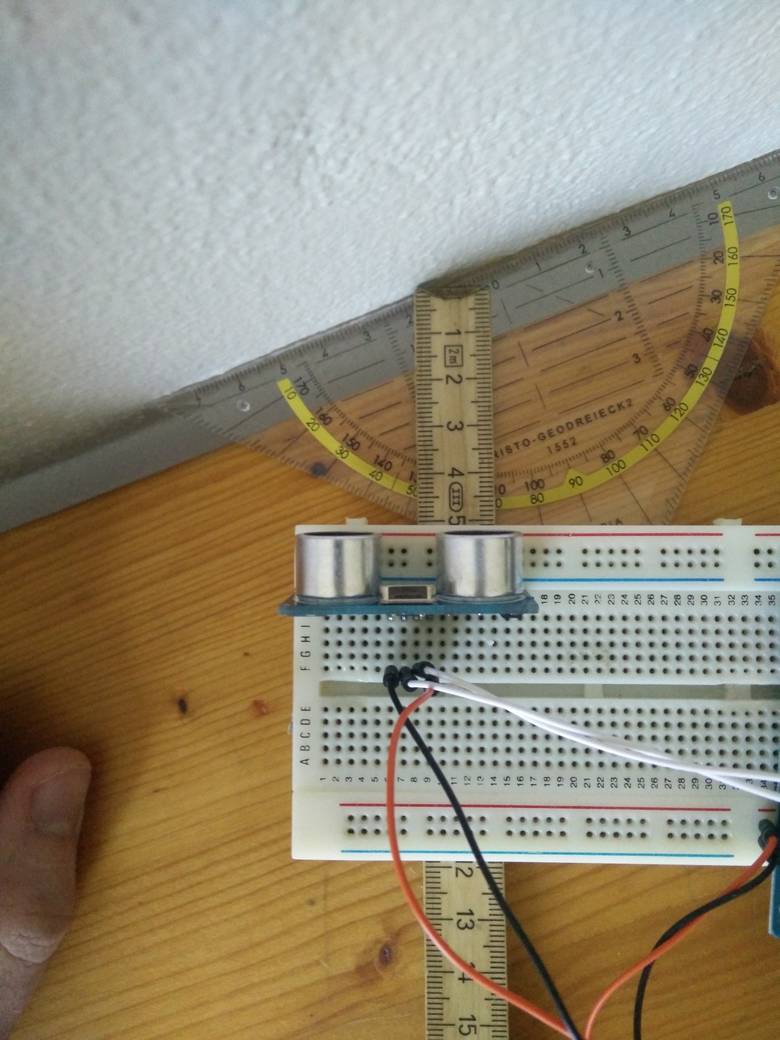
\includegraphics[width=\textwidth]{ultra3.jpg}
    \caption{bla\sinote{ordentlig caption}}
    \label{fig:ultra3}
  \end{subfigure}
\end{figure}
  
\paragraph{Distance}
First the accuracy of the sensors over different distances will be tested. Through this process the minimum and maximum range of the sensors will be discovered. 

\subparagraph{Test Observations}
The results can be seen in \cref{tab:ult_distance}. All three sensors are very close in accuracy to the actual distance. In addition, they do not contradict each other. The minimum distance s 2 cm, and the maximum distance is 565-595 cm, depending on the sensor. A plot of the measurements can be seen in \cref{fig:ult_precision}.

  \begin{table}[htbp]
    \centering
    \begin{adjustbox}{max width=\textwidth}
      \begin{tabular}{c*{15}{c}}
      \toprule
                      & \multicolumn{5}{c}{Sensor 1} & \multicolumn{5}{c}{Sensor 2} & \multicolumn{5}{c}{Sensor 3} \\ 
                        \cmidrule(rl){2-6}             \cmidrule(rl){7-11}            \cmidrule(rl){12-16}
        Distance [cm] & 0\degree of object & 10\degree & 20\degree & 35\degree & 45\degree & 0\degree & 10\degree & 20\degree & 35\degree & 45\degree & 0\degree & 10\degree & 20\degree & 35\degree & 45\degree \\
        \midrule
        0             & 5   & .*  & .   & .   & .   & 5   & .   & .   & . & . & 4   & .   & . & . & . \\ 
        1             & 2   & 2   & 2   & 2   & -   & 2   & 2   & -   & - & - & 2   & 2   & - & - & - \\ 
        2             & 2   & 2   & 3   & 3   & 3   & 2   & 2   & -   & - & - & 2   & 2   & - & - & - \\ 
        3             & 3   & 3   & 3   & 3   & 4   & 3   & 3   & -   & - & - & 3   & 3   & - & - & - \\ 
        4             & 4   & 4   & 4   & 4   & 4   & 4   & 4   & -   & - & - & 4   & 4   & - & - & - \\ 
        5             & 5   & 5   & 5   & 6   & 8   & 5   & 5   & -   & - & - & 5   & 5   & - & - & - \\ 
        10            & 10  & 10  & 9   & 57  & 60  & 10  & 10  & -   & - & - & 10  & 10  & - & - & - \\ 
        20            & 20  & 20  & 19  & 96  & 60  & 20  & 20  & -   & - & - & 20  & 20  & - & - & - \\ 
        40            & 39  & 39  & 38  & 98  & 56  & 39  & 39  & -   & - & - & 39  & 39  & - & - & - \\ 
        80            & 78  & 77  & 74  & 69  & x   & 78  & -   & -   & - & - & 79  & -   & - & - & - \\ 
        160           & 157 & 154 & 148 & 137 & x   & 157 & -   & -   & - & - & 157 & -   & - & - & - \\ 
        320           & 313 & -   & -   & -   & -   & 313 & -   & -   & - & - & 315 & -   & - & - & - \\ 
        450           & 445 & -   & -   & -   & -   & 445 & -   & -   & - & - & 466 & -   & - & - & - \\ 
        570           & 565 & -   & -   & -   & -   & -   & -   & -   & - & - & 566 & -   & - & - & - \\ 
        600           & x   & -   & -   & -   & -   & 595 & -   & -   & - & - & x   & -   & - & - & - \\
        \bottomrule
      \end{tabular}
    \end{adjustbox}
    \caption[Distance test]{Distance test, x marks unstable measurements, and - marks missing. *Does not make sense to measure an angle at 0 distance}\label{tab:ult_distance}
  \end{table}

  \begin{figure}[htbp]
    \centering
    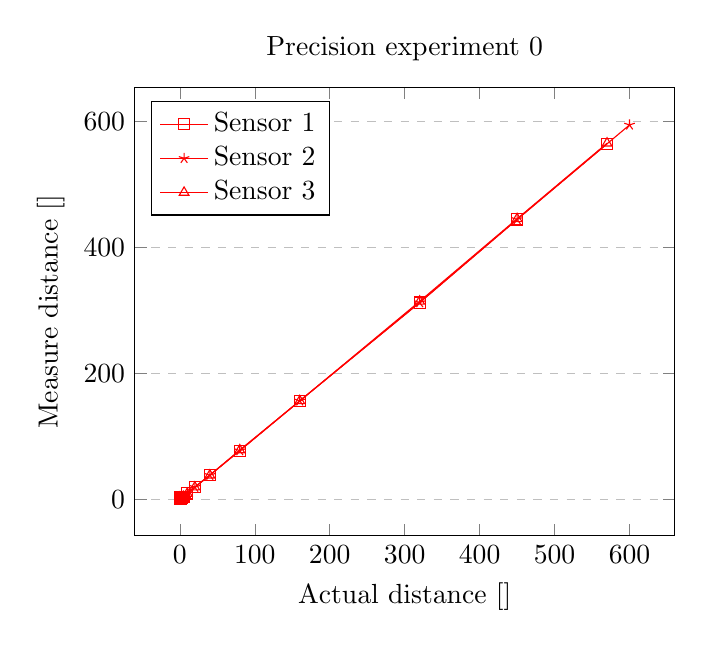
\begin{tikzpicture}    
      \begin{axis}[
                    samples=14,
                    title={Precision experiment 0\degree},
                    xlabel={Actual distance [$\si{\centi\meter}$]},
                    ylabel={Measure distance [$\si{\centi\meter}$]},
                    %xtick={0,1,2,3,4,5,10,20,40,80,160,320,450,570,600},
                    %ytick={0,1,2,3,4,5,10,20,40,80,160,320,450,570,595},
                    %xmode = linear,
                    %ymode = linear, 
                    legend pos= north west,
                    ymajorgrids=true,
                    grid style=dashed
                  ]
        %sensor 1
\addplot[color=red,mark=square]
  coordinates {
              (0,5)
              (1,2)
              (2,2)
              (3,3)
              (4,4)
              (5,5)
              (10,10)
              (20,20)
              (40,39)
              (80,78)
              (160,157)
              (320,313)
              (450,445)
              (570,565)
  };
  \addlegendentry{Sensor 1}
%sensor 2
\addplot[color=red,mark=star]
  coordinates {
              (0,5)
              (1,2)
              (2,2)
              (3,3)
              (4,4)
              (5,5)
              (10,10)
              (20,20)
              (40,39)
              (80,78)
              (160,157)
              (320,313)
              (450,445)
              (600,595)
  };
  \addlegendentry{Sensor 2}
%sensor 3
\addplot[color=red,mark=triangle]
  coordinates {
              (0,4)
              (1,2)
              (2,2)
              (3,3)
              (4,4)
              (5,5)
              (10,10)
              (20,20)
              (40,39)
              (80,79)
              (160,157)
              (320,315)
              (450,446)
              (570,566)
  };
  \addlegendentry{Sensor 3}

      \end{axis}
    \end{tikzpicture}
    \caption[Distance test results]{Distance test at 0 degrees angle, at 570 cm sensor 1 and 3 stopped supplying stable reliable answers.}
    \label{fig:ult_precision}
  \end{figure}
  
\paragraph{Angle}
The angle of the field the sensor measures within is tested, see \cref{tab:ult_angle}. This gives an idea of how directed the sensor is, and thereby at what span the sensor is able to detect an object.

  \begin{table}[htbp]
    \centering
    \begin{adjustbox}{max width=\textwidth}
      \begin{tabular}{c*{13}{c}}
      \toprule
        Distance [cm] & -30\degree & -25\degree & -20\degree & -15\degree & -10\degree & -5\degree & 0\degree & 5\degree & 10\degree & 15\degree & 20\degree & 25\degree & 30\degree \\ 
        \midrule
        15            & x & x  & x & 16 & 16 & 15 & 15 & 15 & 16 & 17 & x  & x & x \\ 
        30            & x & x & 31 & 30 & 30 & 30 & 30 & 30 & 30 & 30 & 31 & x & x \\ 
      \bottomrule
      \end{tabular}
    \end{adjustbox}
    \caption[Sensor angle test]{Sensor angle test. x marks unstable measurements.}
    \label{tab:ult_angle}
  \end{table}

\subparagraph{Test Observations}
The results can be seen in \cref{tab:ult_angle}. The sensors can reliably sense objects within a angle of -20\degree/20\degree.
 
\paragraph{Multiple Ultrasonic Sensors}
If multiple ultrasonic sensors are used in the problem domain at the same time, the sensors may interfere with each other. One sensor is capable of transmitting sound waves to another sensor, which would result in a collision. If this is to be solved, it is important that a collision is detectable or does simply not happen. Getting collision-free measurements requires some coordination between sensors, i.e. who will measure when. An example of a solution is that each sensor is given a timeslot, in which a sensor is allowed to speak, it is important that there is slight delay between each timeslot to ensure that the sound waves has attenuated.